\documentclass[a4paper,11pt]{book}
%\documentclass[a4paper,twoside,11pt,titlepage]{book}
\usepackage{listings}
\usepackage[utf8]{inputenc}
\usepackage[spanish]{babel}
\usepackage{fullpage, mathpazo, amsmath, amsthm, amssymb, amsfonts, nicefrac}
\usepackage{vmargin}

\usepackage{cite}

% \usepackage[style=list, number=none]{glossary} %
%\usepackage{titlesec}
%\usepackage{pailatino}

\decimalpoint
\usepackage{dcolumn}
\newcolumntype{.}{D{.}{\esperiod}{-1}}
\makeatletter
\addto\shorthandsspanish{\let\esperiod\es@period@code}
\makeatother


%\usepackage[chapter]{algorithm}
\RequirePackage{verbatim}
%\RequirePackage[Glenn]{fncychap}
\usepackage{fancyhdr}
\usepackage{graphicx}
\usepackage{afterpage}

\usepackage{longtable}

\usepackage[pdfborder={000}]{hyperref} %referencia

% ********************************************************************
% Re-usable information
% ********************************************************************
\newcommand{\myTitle}{Geometría y Visualización\xspace}
\newcommand{\myDegree}{Máster en Matemáticas\xspace}
\newcommand{\myName}{Jesús Bueno Urbano\xspace}
\newcommand{\myProf}{Carlos Ureña Almagro\xspace}
\newcommand{\myOtherProf}{Pedro A. García Sánchez\xspace}
%\newcommand{\mySupervisor}{Put name here\xspace}
%\newcommand{\myFaculty}{Your Faculty here\xspace}
%\newcommand{\myFacultyShort}{\xspace}
%\newcommand{\myDepartment}{Your department here\xspace}
\newcommand{\myUni}{\protect{Universidad de Granada}\xspace}
%\newcommand{\myLocation}{Granada\xspace}
%\newcommand{\myTime}{\today\xspace}
%\newcommand{\myVersion}{Version 0.1\xspace}


\hypersetup{
pdfauthor = {\myName},
pdftitle = {\myTitle},
pdfsubject = {},
pdfkeywords = {}
pdfcreator = {TeX Live},
pdfproducer = {pdflatex}
}

%\hyphenation{}


%\usepackage{doxygen/doxygen}
%\usepackage{pdfpages}
\usepackage{url}
\usepackage{colortbl,longtable}
\usepackage[stable]{footmisc}
%\usepackage{index}

%\makeindex
%\usepackage[style=long, cols=2,border=plain,toc=true,number=none]{glossary}
% \makeglossary

% Definición de comandos que me son útiles:
%\renewcommand{\indexname}{Índice alfabético}
%\renewcommand{\glossaryname}{Glosario}

\pagestyle{fancy}
\fancyhf{}
\fancyhead[LO]{\leftmark}
\fancyhead[RE]{\rightmark}
\fancyhead[RO,LE]{\textbf{\thepage}}
\renewcommand{\chaptermark}[1]{\markboth{\textbf{#1}}{}}
\renewcommand{\sectionmark}[1]{\markright{\textbf{\thesection. #1}}}

\setlength{\headheight}{1.5\headheight}

\newcommand{\HRule}{\rule{\linewidth}{0.5mm}}
%Definimos los tipos teorema, ejemplo y definición podremos usar estos tipos
%simplemente poniendo \begin{teorema} \end{teorema} ...
\theoremstyle{definition}
\newtheorem{definition}{Definición}[section]
\newtheorem{lemma}{Lema}[section]
 
\theoremstyle{remark}
\newtheorem*{remark}{Nota}

\definecolor{gray97}{gray}{.97}
\definecolor{gray75}{gray}{.75}
\definecolor{gray45}{gray}{.45}
\definecolor{gray30}{gray}{.94}

\lstset{ frame=Ltb,
     framerule=0.5pt,
     aboveskip=0.5cm,
     framextopmargin=3pt,
     framexbottommargin=3pt,
     framexleftmargin=0.1cm,
     framesep=0pt,
     rulesep=.4pt,
     backgroundcolor=\color{gray97},
     rulesepcolor=\color{black},
     %
     stringstyle=\ttfamily,
     showstringspaces = false,
     basicstyle=\scriptsize\ttfamily,
     commentstyle=\color{gray45},
     keywordstyle=\bfseries,
     %
     numbers=left,
     numbersep=6pt,
     numberstyle=\tiny,
     numberfirstline = false,
     breaklines=true,
   }
 
% minimizar fragmentado de listados
\lstnewenvironment{listing}[1][]
   {\lstset{#1}\pagebreak[0]}{\pagebreak[0]}

\lstdefinestyle{CodigoC}
   {
	basicstyle=\scriptsize,
	frame=single,
	language=C,
	numbers=left
   }
\lstdefinestyle{CodigoC++}
   {
	basicstyle=\small,
	frame=single,
	backgroundcolor=\color{gray30},
	language=C++,
	numbers=left
   }

 
\lstdefinestyle{Consola}
   {basicstyle=\scriptsize\bf\ttfamily,
    backgroundcolor=\color{gray30},
    frame=single,
    numbers=none
   }


\newcommand{\bigrule}{\titlerule[0.5mm]}


%Para conseguir que en las páginas en blanco no ponga cabeceras
\makeatletter
\def\clearpage{%
  \ifvmode
    \ifnum \@dbltopnum =\m@ne
      \ifdim \pagetotal <\topskip
        \hbox{}
      \fi
    \fi
  \fi
  \newpage
  \thispagestyle{empty}
  \write\m@ne{}
  \vbox{}
  \penalty -\@Mi
}
\makeatother

\usepackage{pdfpages}
\begin{document}
\begin{titlepage}
 
 
\newlength{\centeroffset}
\setlength{\centeroffset}{-0.5\oddsidemargin}
\addtolength{\centeroffset}{0.5\evensidemargin}
\thispagestyle{empty}

\noindent\hspace*{\centeroffset}\begin{minipage}{\textwidth}

\centering

\includegraphics[width=0.9\textwidth]{images/logo_ugr.png}\\[1.4cm]

\textsc{ \Large TRABAJO FIN DE MÁSTER\\[0.2cm]}
\textsc{Escuela Internacional de Posgrado}\\[1cm]
% Upper part of the page
% 
% Title
{\Huge\bfseries Geometría y visualización\\
}
\noindent\rule[-1ex]{\textwidth}{3pt}\\[3.5ex]
%{\large\bfseries Subtitulo del Proyecto}
\end{minipage}

\vspace{2.5cm}
\noindent\hspace*{\centeroffset}\begin{minipage}{\textwidth}
\centering

\textbf{Autor}\\ {Jesús Bueno Urbano}\\[2.5ex]
\textbf{Directores}\\
{Carlos Ureña Almagro\\
Pedro A. García Sánchez}\\[2cm]

\includegraphics[width=0.3\textwidth]{images/mm.pdf}\\[0.1cm]
\textsc{Máster Universitario en Matemáticas}\\
\textsc{---}\\
Granada, 2018
\end{minipage}
%\addtolength{\textwidth}{\centeroffset}
%\vspace{\stretch{2}}
\end{titlepage}



%\chapter*{}
%\thispagestyle{empty}
%\cleardoublepage

%\thispagestyle{empty}

%\begin{titlepage}
 
\thispagestyle{empty}
\setlength{\centeroffset}{-0.5\oddsidemargin}
\addtolength{\centeroffset}{0.5\evensidemargin}
\thispagestyle{empty}

\noindent\hspace*{\centeroffset}\begin{minipage}{\textwidth}

\centering
%
\includegraphics[width=0.9\textwidth]{images/logo_ugr.png}\\[1.4cm]



 \vspace{3.3cm}

%si el proyecto tiene logo poner aquí

\includegraphics{images/mm.pdf} 
 \vspace{0.5cm}

% Title

{\Huge\bfseries Geometría y visualización\\
}
%\noindent\rule[-1ex]{\textwidth}{3pt}\\[3.5ex]
%{\large\bfseries Subtítulo del proyecto.\\[4cm]}
\end{minipage}

\vspace{2.5cm}
\noindent\hspace*{\centeroffset}\begin{minipage}{\textwidth}
\centering

\textbf{Autor}\\ {Jesús Bueno Urbano}\\[2.5ex]
\textbf{Directores}\\
{Carlos Ureña Almagro\\
Pedro A. García Sánchez}\\[2cm]
%\includegraphics[width=0.15\textwidth]{images/tstc.png}\\[0.1cm]
%\textsc{Departamento de Teoría de la Señal, Telemática y Comunicaciones}\\
%\textsc{---}\\
%Granada, mes de 201
\end{minipage}
%\addtolength{\textwidth}{\centeroffset}
\vspace{\stretch{2}}

 
\end{titlepage}






\cleardoublepage
\thispagestyle{empty}

\begin{center}
{\large\bfseries Geometría y visualización}\\
\end{center}
\begin{center}
Jesús Bueno Urbano\\
\end{center}

%\vspace{0.7cm}
%\noindent{\textbf{Palabras clave}: palabra\_clave1, palabra\_clave2, palabra\_clave3, ......}\\

\vspace{0.7cm}
\noindent{\textbf{Resumen}}

En este Trabajo Fin de Máster hemos querido hacer un recorrido por los conceptos básicos de del Ray Tracing para poder representar y visualizar superfícies implícitas. Para ello en el  primer capítulo haremos un repaso sobre métodos elementales para implicitar superficies, es decir, para poder transformar una expresión no implícita, paramétrica en nuestro caso, de una superficie en la expresión implícita de ésta. Sobre todo nos centraremos en el método de la base de Gröbner y presentaremos los métodos de la resultante y de Wu-Ritt.

Ya en el segundo capítulo el tema principal de éste será buscar métodos de visualización de superficies como la poligonalización de superficies, en particular, presentaremos un algoritmo de triangulación extraído de \cite{Hartmann03}. A continuación explicaremos el concepto de Ray Tracing.

A continuación haremos una introducción al Análisis de Intervalos y a sus propiedades, a los Intervalos Modales y a las llamadas extensiones semánticas. Todo esto nos servirá para, finalmente, aplicarlo al Ray Tracing y así presentar varios algoritmos mejorados cuya eficiencia compararemos.
\cleardoublepage


%\thispagestyle{empty}


%\begin{center}
%{\large\bfseries Project Title: Project Subtitle}\\
%\end{center}
%\begin{center}
%First name, Family name (student)\\
%\end{center}

%\vspace{0.7cm}
%\noindent{\textbf{Keywords}: Keyword1, Keyword2, Keyword3, ....}\\

%\vspace{0.7cm}
%\noindent{\textbf{Abstract}}\\

%Write here the abstract in English.

\chapter*{}
\thispagestyle{empty}

\noindent{\rule[-1ex]{\textwidth}{2pt}\\[4.5ex]}
Yo, \textbf{Jesús Bueno Urbano}, estudiante del Máster Universitario en Matemáticas de la \textbf{Escuela Internacional de Posgrado de la Universidad de Granada}, con DNI 20078941X, autorizo que la siguiente copia de mi Trabajo Fin de Máster pueda ser consultada por las personas que lo deseen.

\vspace{2cm}


\includegraphics[scale=0.3]{images/firma.png}

\vspace{1cm}

\noindent Fdo: Jesús Bueno Urbano

\vspace{2cm}

\begin{flushright}
En Granada, a \today.
\end{flushright}


\chapter*{Agradecimientos}
\thispagestyle{empty}
\vspace{1cm}

Agradecimientos aquí.
\frontmatter
\tableofcontents %Buscar como eliminar ese número romano
%\listoffigures
%\listoftables
%
\mainmatter
\setlength{\parskip}{5pt}

\chapter{Implicitación de superficies}

\section{Introducción}

Las superficies implícitas se usan en la Ciencia de Computación Gráfica desde los años 70 para modelar objetos geométricos, pero su uso e importancia han ido creciendo en años recientes ya que pueden ser usadas para describir objetos en espacios de dimensión arbitraria. En este Trabajo Fin de Máster nos centraremos en objetos de dimensión dos y tres. En muchas ocasiones, un mismo objeto matemático se puede definir de una forma particular, por tanto nos cabe preguntarnos por qué las superficies en forma implícita se han popularizado tanto. La respuesta la encontramos en que la expresión implícita de una superficie, en contraste con la definición paramétrica del de la misma, suele ser compacta, manejable y es trivial comprobar la pertenencia de un punto al objeto dado. Por ejemplo, una expresión paramétrica de la esfera unidad es
$$X(u,v) = (\cos(u)\sin(v),\sin(u)\sin(v),\cos(v)), \hspace{0.5cm} (u,v) \in [0,2\pi] \times [0,\pi],$$
mientras que su expresión en forma implícita es
$$f(x,y,z) = x^2 + y^2 + z^2 - 1.$$

Aunque hemos mencionado algunas ventajas de usar la forma implícita para la modelización y visualización de superficies, su principal debilidad es la cantidad de tiempo que necesitan para la visualización directa, por ejemplo usando Ray Tracing\cite{Groot05}. Otra de las debilidades de las superficies en forma implícita es la dificultad de controlar la forma de las superficies durante una visualización rápida en un entorno interactivo. Esto lleva a que las representaciones paramétricas sigan siendo populares hoy en día gracias a la relativamente rápida renderización que presentan.

Aún presentando estas debilidades, las superficies en forma implícita son una forma flexible de crear objetos complejos ya que ofrecen una clasificación manejable y clara de conjuntos de puntos, es decir, es fácil saber si un punto del espacio se encuentra{ \em dentro},{ \em fuera} o{ \em en} la superficie.

Además también se pueden usar para la representación de nubes de puntos. Por ejemplo, en imágenes de datos médicos y reconstrucción de objetos representados como medias de conjuntos de puntos\cite{Benedet05,Peiro06}. En \cite{Uhlir03} se describe el llamado{ \em método RBF} basado en técnicas variacionales donde, dados una serie de puntos de una superficie $S$ de la cual no conocemos su expresión, procedemos a calcular una función en forma implícita que modele una superficie $S'$ que sea una aproximación razonable de la superficie inicial e interseque a los puntos que conocemos.

\section{Descripción del problema}

Una representación implícita de una superficie $S$ se define como el conjunto de puntos $p \equiv (x,y,z) \in \mathbb{R}^3$ que son solución de la ecuación $f(p) = 0$, donde $f : \mathbb{R}^3 \to \mathbb{R}$ es una función que asigna un valor escalar a cada punto del espacio. Es decir,
$$S = \{ p \in \mathbb{R}^3 : f(p) = 0 \}.$$

Sea el sólido $A$ el espacio descrito por la preimagen de la función $f$ en $]-\infty,0]$. Por uniformidad consideraremos el siguiente criterio:
$$\begin{tabular}{l c l}
    $p \in \interior(A)$ & si & $f(p) < 0$, \\
    $p \in \partial A$ & si & $f(p) = 0$, \\
    $p \in \exterior(A)$ & si & $f(p) > 0$.
\end{tabular}$$
Donde $\interior(A)$, $\partial A$ y $\exterior(A)$ denotan el interior, frontera y exterior de $A$ respectivamente. Esto establece por medio de la vía topológica que la función implícita es negativa en el{ \em interior}, cero en la superficie, véase{ \em frontera}, y positiva en el{ \em exterior}\cite{Hart01}.

Este sistema es un estándar que se suele usar por comodidad y por ser el más común entre la literatura de este tipo de trabajos. Otros ejemplos incluyen a \cite{Uhlir03} o \cite{Blinn82} donde las funciones implícitas definidas eran positivas en el interior y negativas en el exterior del sólido, o por ejemplo \cite{Ricci73} donde eran siempre positivas y alcanzaban el valor unidad en la superficie, menos uno en el interior y mayor que uno en el exterior.

Está claro que estas definiciones no afectan al problema principal, véase que, volviendo al ejemplo de la esfera, en \cite{Uhlir03} usan lo que llaman la forma inversa que sería
$$f(x,y,z) = - x^2 - y^2 - z^2 + 1.$$

Ahora que hemos descrito las ventajas de las superficies dadas de forma implícita queremos ver los métodos para crear la representación implícita de objetos arbitrarios.

Hay infinidad de métodos para la realizar la implicitación de superficies, algunos ya los hemos mencionado como los basados en nubes de puntos y/o técnicas variacionales, pero aquí nos centraremos en los métodos de eliminación de variables que parten de expresiones paramétricas de la superficie, o parte de a superficie, para después modificarlas y así obtener una expresión implícita de ésta mediante operaciones simbólicas.

\section{Métodos de eliminación de variables}

Eliminación es una disciplina matemática para suprimir variables de sistemas de ecuaciones polinomiales. En nuestro caso este método se aplica a la parametrización de la superficie que se expresa como una sistema de ecuaciones
\begin{equation}
    \begin{tabular}{c c c}
        $x_1$ & = & $f_1(t_1, \dotso, t_m)$, \\
         & $\vdots$ & \\
        $x_n$ & = & $f_n(t_1, \dotso, t_m).$
    \end{tabular}
    \nonumber
\end{equation}
En donde las funciones $f_i$ son polinomios o funciones racionales de éstos.

El método consiste encontrar las relaciones entre las variables y, así pues, la ecuación implícita que nos expresa la misma superficie que el sistema de ecuaciones de su expresión paramétrica.

En \cite{Hoffmann93} se hace una clasificación del método de la resultante, el método de la base de Gröbner y el método de Wu-Ritt. Todos los métodos que vamos a describir tienen una propiedad común y ésta es que el resultado del algoritmo es una ecuación que puede ser utilizada por métodos de visualización directa.

\subsection{Método de la base de Gröbner}

Este método se basa en encontrar una base de Gröbner para un ideal $I$, donde éste es un conjunto de polinomios que cumple con el requisito de existencia de una base de Gröbner. La búsqueda  de una base de Gröbner reducida se basa en la búsqueda de una solución exacta de un sistema de ecuaciones polinomiales. Si el sistema de ecuaciones polinomiales tiene una solución, entonces las variables del sistema son eliminadas y el conjunto original de ecuaciones se transforma. Este nuevo conjunto de ecuaciones transformadas sí puede ser solucionado de forma sencilla.

La transformación de la expresión paramétrica en un expresión implícita puede ser resuelto de una forma satisfactoria usando una base de Gröbner de un ideal. Las parametrizaciones que tenemos como entrada pueden ser tanto polinomiales como racionales.

\subsubsection*{Ideal}

Un subconjunto $I \subset k[x_1, \dotso, x_n]$ se dice ideal en $k[x_1, \dotso, x_n]$ si se verifican las siguientes dos condiciones.
\begin{enumerate}
    \item Si $f, g \in I$, entonces $f + g \in I$.
    \item Si $f \in I$, entonces $fg \in I$ para todo $g \in k[x_1, \dotso, x_n]$.
\end{enumerate}

Sean $f_1, \dotso, f_s \in k[x_1, \dotso, x_n]$, el conjunto $I =  \left\{ \sum_{i=1}^{s} g_i f_i \ : \ g_i \in k[x_1, \dotso, x_n] \right\}$ es un ideal de $k[x_1, \dotso, x_n]$ y además es el menor ideal que contiene a los polinomios $f_1, \dotso, f_s$. El conjunto $\left\{ f_1, \dotso, f_s \right\}$ se llama conjunto generador o base del ideal $I$. 

\subsubsection*{Ordenamiento de los polinomios}

Para la computación de la base de Gröbner, necesitamos el concepto de orden monomial.

\begin{definition}
    Un orden monomial se define como un orden total sobre el conjunto de los monomios en un anillo polinomial verificando esta propiedad respecto del producto, i.e., dados dos monomios $u$ y $v$ tales que $u \leq v$ y sea $w$ otro monomio, entonces $uw \leq vw$.
\end{definition}

En el caso de una cantidad finita de variables se tiene la siguiente forma equivalente.

\begin{definition}
    Un orden sobre el conjunto de monomios en un anillo polinomial se dice monomial si se verifican las siguientes condiciones:
    \begin{itemize}
        \item El orden es total.
        \item Si $u$ es un monomio cualquiera se tiene que $1 \leq u$.
    \end{itemize}
\end{definition}

Aunque existen varios órdenes monomiales, y se pueden escoger según la situación, los más comunes son los siguientes.

\textit{Orden lexicográfico}

Dado el conjunto de monomios en $n$ variables $x_1, \dotso, x_n$ tales que establecemos que $x_1 \prec x_2 \prec \dotso \prec x_n$ el orden lexicográfico se define como
$$1 \prec x_1 \prec x_1^2 \prec \dotso \prec x_2 \prec x_1 x_2 \prec x_1^2 x_2 \prec \dotso \prec x_2^2 \prec x_1x_2^2 \prec \dotso \prec x_n \prec \dotso $$

\textit{Orden lexicográfico graduado}

A diferencia del método anterior, este método primero ordena los términos por su grado y los términos de igual grado se ordenan de manera lexicográfica. Tomando el ejemplo anterior nos quedaría:
$$1 \prec x_1 \prec x_2 \prec \dotso \prec x_n \prec x_1^2 \prec x_1 x_2 \prec x_1x_2 \prec \dotso\prec x_1x_n \prec x_2^2 \prec x_2x_3 \prec \dotso$$

\subsubsection*{Reducción polinomial}

Para calcular la base de Gröbner es importante elegir un orden $\prec$, por ello tras haberlo elegido pasamos a definir los siguientes términos.

\begin{definition}
Para cada polinomio $f(x_1, \dotso, x_n)$ se define el monomio líder como el mayor término de $f$ bajo $\prec$ con coeficientes no nulos. Se denota por $LM(f)$.
\end{definition}

\begin{remark}
El coeficiente del monomio líder se llama coeficiente líder y se denota por $LC(f)$.
\end{remark}

\begin{definition}
El término líder de un polinomio $f$ se define como el producto del monomio líder. Se denota por $LT(f)$.
\end{definition}

\begin{definition}
La cola de un polinomio $f(x_1, \dotso, x_n)$, denotado por $TT(f)$ se obtiene separando el término líder del resto del polinomio.
\end{definition}

Con las definiciones dadas se puede reescribir un polinomio $f(x_1, \dotso, x_n)$ como
$$f = LT(f) + TT(f).$$
Ahora podemos proceder a la reducción polinomial propiamente dicha.

Dados dos polinomios $f(x_1, \dotso, x_n)$ y $g(x_1, \dotso, x_m)$ se dice que $g$ reduce a un polinomio $h$ respecto de $f$ si, y sólo si, $LT(g)$ se puede eliminar mediante la resta de un múltiplo apropiado de $f$. Esta operación se denota por $g \to_f h$.
Por tanto, la reducción $g \to_f h$ es posible si, y sólo si, existe un escalar $b$ y un monomio $u$ tales que $h = g - buf$ donde $b = \frac{LC(g)}{LC(f)}$ y $u =\frac{LM(g)}{LM(f)}$.

Se dice que un polinomio $g$ se reduce respecto de un conjunto, o base, de polinomios $F = \{ f_1, \dotso, f_n \}$ si $g$ es reducible respecto de uno o más polinomios de $F$. En tal caso la reducción de un polinomio puede conducir a una secuencia de reducciones, lo que es un proceso finito. Se puede probar además que cada polinomio $g_i$ en la secuencia de reducciones y el propio polinomio $g$ es un elemento del ideal $(f_1, \dotso, f_n)$.

\subsubsection*{S-polinomios}

Este proceso que hemos llevado a cabo nos conduce al concepto de \textbf{S-polinomios}. Para dos polinomios $f$ y $g$ se define su S-polinomio como:
$$S(f,g) = \frac{x^{\gamma}}{LT(f)} \cdot f - \frac{x^{\gamma}}{LT(g)} \cdot g.$$
Donde $x^{\gamma}$ representa el máximo común divisor entre los monomios líderes de $f$ y $g$.

\subsubsection*{Base de Gröbner}

Después de escoger un orden, el conjunto $G = \{ g_1, \dotso, g_l \}$ del ideal $I$ es una base de Gröbner si
$$\langle LT(g_1), \dotso, LT(g_l) \rangle = \langle LT(I) \rangle.$$
Es decir, el conjunto $G \subset I$ es la base de Gröbner si, y sólo si, el término líder de cualquier elemento de $I$ es divisible entre $LT(g_i)$ para algún $i = 1, \dotso, l$. En consecuenia una base de Gröbner de un conjunto de polinomios es un tipo concreto de base del ideal que generan que cumple:
\begin{itemize}
    \item Todo polinomio en el ideal se reduce a cero respecto a la base.
    \item Todo polinomio tiene una única forma normal respecto de la base.
\end{itemize}

Cuando la parametrización se compone de funciones polinomiales, ésta se puede expresar como
\begin{equation}
\begin{tabular}{c c c}
$x_1$ & $=$ & $f_1(t_1, \dotso, t_m)$, \\
 & $\vdots$ &  \\
$x_n$ & $=$ & $f_n(t_1, \dotso, t_m)$.
\end{tabular}
\nonumber
\end{equation}
Donde $f_1, \dotso, f_n$ son polinomios en $K[t_1, \dotso, t_m]$ con $K$ un cuerpo.

Este sistema se puede ver como la proyección $F : K^m \to K^n$ definida por
$$F(t_1,\dotso, t_m) = (f_1(t_1,\dotso, t_m), \dotso, f_n(t_1,\dotso, t_m)).$$

Entonces, la imagen es un subconjunto de $K^n$ parametrizado por el sistema previo. Teniendo en cuenta que $F(K^m)$ no es una variedad afín, se obtiene que la solución del problema de conversión de ecuaciones paramétricas a implícitas es equivalente a encontrar la variedad mínima que contiene a $F(K^m)$, i.e., el problema de implicitación consiste en la eliminación de parámetros de la descripción paramétrica. La ecuación final contiene solo las variables $x_1, \dotso, x_n$.
\\La eliminación de variables se puede realizar calculando la base de Gröbner reducida para un ideal $I = \langle x_1 - f_1, \dotso, x_n - f_n \rangle$. Para enfrentarse a este problema solo es necesario tener en cuenta el orden $\prec$.

El segundo método es la implicitación racional, la cual puede ser expresada como
\begin{equation}
\begin{tabular}{c c c}
$x_1$ & $=$ & $\frac{f_1(t_1, \dotso, t_m)}{g_1(t_1, \dotso, t_m)}$, \\
 & $\vdots$ &  \\
$x_n$ & $=$ & $\frac{f_n(t_1, \dotso, t_m)}{g_n(t_1, \dotso, t_m)}$.
\end{tabular}
\nonumber
\end{equation}
Donde $f_1, \dotso, f_n, g_1, \dotso, g_n \in K[t_1, \dotso, t_m]$.

Sabemos que $F : K^m \to K^n$ no se puede definir en todo $K^m$ ya que, obviamente, hay que excluir el conjunto de raíces de los polinomios $g_i$ para todo $i = 1, \dotso, n$. Si denotamos como $W \subset K^m$, entonces
$$F(t_1, \dotso, t_m) = \left( \frac{f_1(t_1, \dotso, t_m)}{g_1(t_1, \dotso, t_m)}, \dotso, \frac{f_n(t_1, \dotso, t_m)}{g_n(t_1, \dotso, t_m)}  \right)$$
define la proyección $F : K^m \setminus W \to K^n$.

El objetivo es encontrar la variedad mínima en $K^n$ que contenga $F(K^m / W)$. En la parametrización definida se eliminan las fracciones multiplicando la iésima coordenada por el polinomio $g_i$. Entonces la ecuación $1 - g_1 \dotso g_n y = 0$, para polinomios $g_i$ no nulos en la variedad definida, se añade  y se evalúa la base de Gröbner reducida. Los elementos de la base de Gröbner que no contienen a las variables $t_1, \dotso, t_n, y$ definen la representación implícita de la variedad afín dada.
\\Una explicación más exhaustiva se puede encontrar en \cite{Hoffmann93}.

\subsubsection*{Ejemplo}

\begin{figure}[h]
\centering
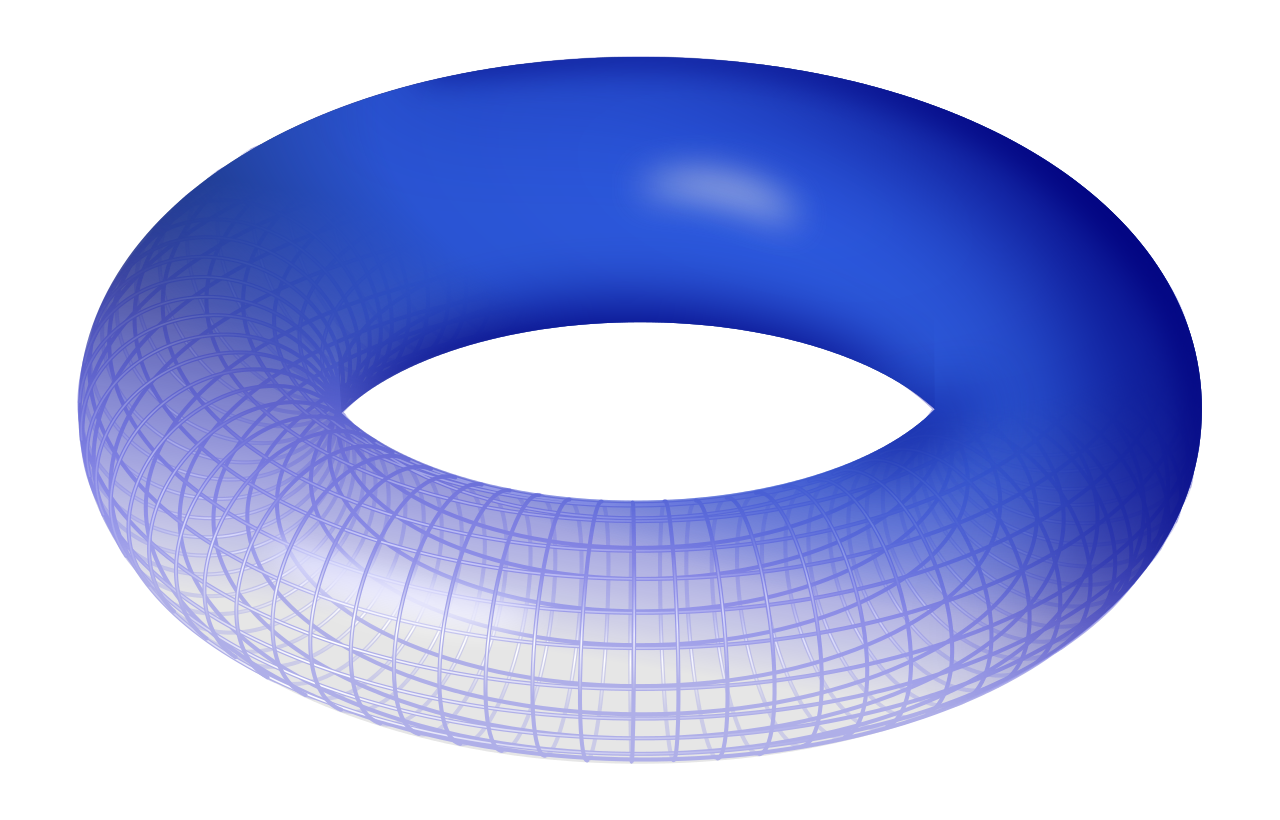
\includegraphics[width=0.5\linewidth]{images/Torus.png}
\caption{Representación clásica de un toro. Imagen extraída de \cite{Wikipedia:Torus}.}
\end{figure}

La expresión paramétrica de un toro es
\begin{equation}
\begin{tabular}{c c l}
$x$ & $=$ & $r \cos u \cos t + R \cos t$, \\
$y$ & $=$ & $r \cos u \sin t + R \sin t$, \\
$z$ & $=$ & $r \sin u$.
\end{tabular}
\nonumber
\end{equation}

Si renombramos esta expresión como
\begin{equation}\label{Uhlir03-14}
c_u = \cos u, \hspace{0.5cm} c_t = \cos t, \hspace{0.5cm} s_u = \sin u \hspace{0.5cm} \text{y} \hspace{0.5cm} s_t = \sin t,
\end{equation}
podemos representar la expresión paramétrica inicial en polinomios como
\begin{equation}\label{Uhlir03-15}
\begin{tabular}{r c c}
$x - r c_u c_t - R c_t$ & $=$ & $0$, \\
$y - r c_u s_t - R s_t$ & $=$ & $0$, \\
$z - r s_u$ & $=$ & $0$.
\end{tabular}
\end{equation}
Añadiendo las identidades
\begin{equation}
\begin{tabular}{r c c}
$c_u^2 + s_u^2 - 1 = 0$ & $=$ & $0$, \\
$c_t^2 + s_t^2 - 1 = 0$ & $=$ & $0$.
\end{tabular}
\end{equation}
La base de Gröbner reducida para el ideal $I$, generado por los polinomios (\ref{Uhlir03-14}) y (\ref{Uhlir03-15}), contiene 9 elementos. Uno solo de estos elementos no contiene variables en $c_u, s_u, c_t \text{ ó } s_t$, y tiene la forma
$$(x^2 + y^2 + z^2 - r^2 - R^2)^2 = 4 R^2 (z^2 - r^2),$$
la cual es la expresión implícita del toro.

\subsection{Método de la resultante}

El término { \em resultante} se suele introducir si se presenta la siguiente cuestión: ¿Cuándo dos polinomios en el anillo de polinomios $K[x]$ tienen un divisor común? Los métodos que usan la evaluación de la resultante se pueden usar para eliminar un subconjunto de variables del sistema inicial de ecuaciones algebraicas no lineales.
Un dato interesante de la resultante para polinomios en varias variables es que para $n+1$ polinomios ésta elimina $n$ variables a la par. A diferencia del método de la base de Gröbner, este método es no secuencial. La idea básica que subyace en las resultantes multidimensionales es la conversión de un problema de eliminación no lineal en uno lineal, lo cual ayuda a aplicar métodos conocidos de Álgebra Lineal para resolver el sistema.

Existen distintos tipos de resultante. La definición básica involucra dos polinomios en una variable, por ejemplo la resultante de Sylvester o Bézout, y a partir de ahí se puede ir generalizando a dos polinomios en dos variables y después a tres polinomios en dos variables, la resultante de Dixon. Esta última puede generalizarse a $n+1$ polinomios en $n$ variables. Aquí daremos una simple pincelada para dar la idea de las resultantes ya nombradas. Podemos encontrar más información en \cite{Berchtold00}.

\subsubsection*{Resultante de Sylvester}

El principal problema es la tendencia a encontrar si dos polinomios $f, g \in K[x]$ tienen divisor común. Existen varias maneras de encontrarlo, por ejemplo, el algoritmo de Euclides se puede usar para descomponer los polinomios en productos de factores simples. O por ejemplo, el siguiente lema.

\begin{lemma}
	Sean $f,g \in K[x]$ tales que $deg(f) = n > 0$ y $deg(g) = m > 0$. Se tiene que $f$ y $g$ tienen un divisor común si y sólo si existen polinomios $A, B \in K[x]$ verificando que
	\begin{enumerate}
		\item ambos polinomios $A$ y $B$ son no nulos,
		\item $A$ y $B$ tienen como mínimo grado $m-1$ y $n-1$ respectivamente y
		\item $Af + Bg = 0$.
	\end{enumerate}
\end{lemma}

\begin{definition}
	Sean $f, g \in K[x]$ dados como $f = a_n x^n + \dots + a_0$ y $g = b_m x^m + \dots + b_0$ donde $a_n, b_m \neq 0$, entonces la resultante de Sylvester de $f$ y $g$ es de la forma
$$\operatorname{Res}(f,g) = \operatorname{Det}(\operatorname{Syl}(f,g)).$$
Donde $\operatorname{Syl}(f,g)$ denota
	$$\begin{pmatrix}
	a_n & & & & & b_m & & & & \\
	a_{n-1} & a_n & & & & b_{m-1} & b_m & & & \\
	a_{n-2} & a_{n-1} & a_n & & & b_{m-2} & b_{m-1} & b_m & & \\
	\vdots & \vdots & & \ddots & \vdots & \vdots & \vdots & \vdots & \ddots & \\
	a_1 & \dotso & \dotso & \dotso & a_{n} & b_1 & \dotso & \dotso & \dotso & b_{m} \\
	a_0 & \dotso & \dotso & \dotso & a_{n-1} & b_0 & \dotso & \dotso & \dotso & b_{m-1} \\
	 & a_0 & \dotso & \dotso & a_{n-2} & & b_0 & \dotso & \dotso & b_{m-2} \\
	 & & \ddots & \vdots & \vdots & & & \ddots & \vdots & \vdots \\
	 & & & a_1 & a_0 & & & & b_1 & b_0 \\
	 & & & & a_0 & & & & & b_0
	\end{pmatrix}$$
y los espacios en blanco de la matriz denotan ceros.
\end{definition}

Ahora realizaremos un ejemplo sencillo para comparar este método con el de la base de Gröbner.

Sean por ejemplo los polinomios:
$$f = x^2 y - 1, \hspace{2cm} g = x^2 + y^2 + xy - 4.$$

Aplicando el método de la resultante de Sylvester tenemos
$$\operatorname{Res}(f,g) = \operatorname{Det} \begin{pmatrix}
y & 0 & 1 & 0 \\
0 & y & y & 1 \\
-1 & 0 & y^2 - 4 & y \\
0 & -1 & 0 & y^2 - 4
\end{pmatrix} = y^6 - 8y^4 + y^3 + 16y^2 - 8y + 1.$$

Para comparar podemos ver la solución obtenida mediante el método de la base de Gröbner para el ideal $I = \langle f,g \rangle$ cuya base de Gröbner reducida respecto del orden lexicográfico sería
$$\langle x - 4y^5- y^4 + 32y^3 + 4y^2 - 64y + 16 , y^6 - 8y^4 + y^3 + 16y^2 - 8y + 1 \rangle.$$

\subsubsection*{Resultante de Bézout}

Es similar a la resultante de Sylvester, salvo que la definición de matriz de Bézout es un poco más dificultosa que ésta, pero a cambio ésta tiene dimensión $n \times n$ en lugar de la dimensión $(n+m) \times (n+m)$. En consecuencia, la evaluación del determinante de la matriz Bézout es mucho más rápido.

\subsubsection*{Resultante de Dixon}

Es una versión generalizada de la resultante y matriz de Bézout para tres polinomios en dos variables. Entonces la resultante de Dixon se generaliza para $n+1$ polinomios en $n$ variables.

\subsection{El método de Wu-Ritt}

En esta sección daremos una breve introducción a la teoría de este método. Éste se basa en la aproximación de Wu-Ritt para encontrar un conjunto característico para un sistema de ecuaciones no lineales. Dado un sistema de ecuaciones polinomiales $S = \{ f_1, \dotso, f_m \}$ se transforma en una forma triangular $S'$. Es importante notar que si el número $n$ de variables es mayor que el número de ecuaciones del conjunto $S$, entonces el conjunto de variables se divide en dos subconjuntos: las variables independientes, que denotaremos por $\{ u_1, \dotso, u_k \}$, y las dependientes, que denotaremos por $\{ y_1, \dotso, y_l \}$.

La pseudodivisión de polinomios de varias variables es la operación clave en la computación de conjuntos característicos. Para realizar la pseudodivisión se da uso de la representación recursiva de los polinomios con lo cual se define la siguiente reducción polinomial.

Un polinomio $f_i$ se reduce respecto de otro polinomio $f_j$ si verifican una de las dos siguientes condiciones:
\begin{enumerate}
\item La mayor variable de $f_i$ es menor, con respecto a $\prec$ , que la mayor variable de $f_j$.
\item El grado de la mayor variable en $f_j$ es mayor que el grado de la mayor variable en $f_i$.
\end{enumerate} 

Si $f_i$ no es reducible respecto de $f_j$, entonces $f_i$ se reduce a $r$ mediante la pseudodivisión entre $f_j$.

\begin{definition}
	Dado un conjunto finito $\Sigma$ de polinomios $u_1, \dotso, u_k, y_1, \dotso, y_l$ un conjunto característico $\Phi$ de $\Sigma$ se define de cualquiera de las siguientes maneras:
	\begin{enumerate}
		\item $\{ g_1 \}$ donde $g_1$ es un polinomio de $\{ u_1, \dotso, u_k \}$.
		\item Una cadena $\langle g_1, \dotso, g_l \rangle$ donde cada $g_i$ es un polinomio en $\{ u_1, \dotso, u_k, y_1, \dotso, y_i \}$, con coeficiente líder $LC(g_i)$, tales que:
		\begin{itemize}
			\item Cualquier cero de $\Sigma$ es un cero de $\Phi$.
			\item Cualquier cero de $\Phi$ que no es cero de ninguno de los coeficientes líderes $LC(g_i)$ es un cero de $\Sigma$.
		\end{itemize}
	\end{enumerate}
\end{definition}
Podemos encontrar más información sobre el presente método en \cite{Berchtold00}, \cite{Gallo91_2} o \cite{Gallo91_1}.

\section{Conclusiones}

Todos los métodos mencionados tienen una característica común: si hacemos uso de ellos para convertir la expresión paramétrica de un objeto a la expresión implícita de éste entonces lo que obtenemos es una sola ecuación. A partir de ahí las superficies pueden ser visualizadas con métodos de visualización directa.

Por supuesto, esto es solo un tipo de métodos de implicitación de superficies, ya que existe una  gran variedad. Alguno ya ha sido mencionado al comienzo de este capítulo y otros pueden ser consultados en la bibliografía. En este tipo de métodos no es necesario conocer la expresión paramétrica del objeto.
\chapter{Representación y visualización de superficies implícitas}

Escribir introducción.

\section{Representación de superficies algebraicas y blobs}

\subsection{Superficies algebraicas}

Una superficie se dice algebraica si se define por polinomios cuyo grado indica el grado de la superficie. El grado indica el número de intersecciones de la superficie y una recta.\cite{Bloomenthal97} Por ejemplo un plano tiene grado 1 mientras que una esfera tiene grado 2. El uso de polinomios tiene la ventaja de ser menos costoso, en tiempo de renderización, que cualquier otra representación analítica general.
\par Las superficies algebraicas más comunes son las cuadráticas. Este tipo de superficies son fáciles de renderizar son muy pocos parámetros para controlar su forma, además, es posible usar coordinadas homogéneas para aplicar transformaciones afines. A continuación mostramos típicas superficies cuadráticas como son la esfera, el cilindro y el cono.

\begin{figure}[h]
	\centering
	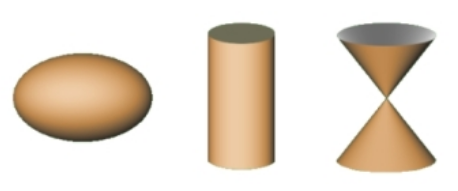
\includegraphics[scale=0.7]{images/florez4.png}
	\caption{Ejemplos básicos de superficies cuadráticas.}
\end{figure}

\subsection{Blobs}

Los blobs son sumas de distribuciones gaussianas inspiradas en la distribución de densidad de las moléculas. Este tipo de superficies fueron usadas por primera vez por Blinn \cite{Blinn82} para renderizar una animación del ADN para el programa de televisión Cosmos de Carl Sagan en donde cada átomo era aproximado por una esfera gaussiana.
\par La suma de esferas gaussianas genera una unión entre las superficies. Blinn propuso la función

\begin{equation}
f(x,y,z) = \sum_{i=1}^{n} b_i e^{-a_i r_i^2} - 1
\nonumber
\end{equation}

donde cada función está centrada en un término $r$. El término $r$ se calcula como $r(x,y,z) = \sqrt{(x - x_i)^2 + (y-y_i)^2 + (z-z_i)^2}$. El término $b$ representa la altura de la función y el término $a$ es la desviación estándar. El efecto de la función blob se puede modificar cambiando los parámetros.

\begin{figure}[h]
	\centering
	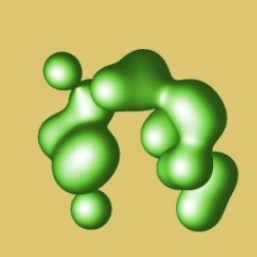
\includegraphics[scale=0.7]{images/florez3.png}
	\caption{Ejemplo de sumas de esferas gaussianas.}
\end{figure}

La función exponencial define una esfera gaussiana que tiende a infinito a la par que la exponencial tiende a cero. Esto significa que cada esfera gaussiana influye sibre las demás sin importar la separación que exista entre ellas. Los objetos flexibles\cite{Wyvill86} computan als esferas usando aproximaciones polinomiales.

\section{Métodos de visualización}

En esta sección cubrimos dos de los métodos de visualización usados y referenciados en la bibliografía de superficies implícitas de forma más frecuente: Poligonalización y ray tracing. Cubriremos ambos con detalle, pero cabe destacar que en el resto del Trabajo Fin de Máster nos centraremos en el desarrollo del segundo.

\subsection{Poligonalización de superficies implícitas}

La idea general de los métodos de poligonalización consiste en la creación de polígonos que representen la superficie implícita. Los polígonos son fáciles de renderizar en los sistemas gráficos modernos, por tanto, este método suele ser el elegido cuando necesitamos de visualización interactiva.
\par Existen varios métodos  de poligonalización de superficies, siendo los más populares:

\begin{itemize}
	\item El llamado{ \em método de las celdas fijas}\cite{Bloomenthal90} consistente en dividir el espacio en poliedros de forma conveniente (cubos, tetraedros,...) y, tras esto, en calcular la intersección de la superficie con  las aristas de los poliedros para así definir los vértices de la poligonalización. Estos vértices han de ordenarse para crear poígonos convexos.
	\par Obviamente la calidad del resultado depende en gran medida de como de { \em fina} sea la división del espacio, esto es, si los poliedros son demasiado grandes entonces se perderan una gran cantidad de detalles y si son demasiado pequeños crearán polígono en exceso que realentizarán la renderización.
	\par Este problema se puede solucionar con una serie de métodos adaptativos donde el tamaño de la celda según el detalle de la superficie, véase, si en una zona nos interesa hacer una poligonalización más detallada allí habrá una división más fina. Aunque estos métodos son difíciles de implementar y aún no son muy populares por esta razón y las celdas de tamaño fijo suelen ser la opción más común.
	\item El segundo método más común son los{ \em marching methods} que consisten en crear, de forma sucesiva, un mallado triangular comenzando con un punto o un polígono dado. Este método lo explicaremos mejor a continuación con un ejemplo claro donde explicaremos un algoritmo concreto extraído de \cite{Hartmann03}.
\end{itemize}

\begin{remark}
	El siguiente algoritmo está extraído de \cite{Hartmann03}, pero al aparecer en \cite{Hartmann98} los derechos pertenecen a Springer-Verlag.
\end{remark}

\subsection{El algoritmo de triangulación}

La formulación del algoritmo de triangulación no usa ninguna representación especial de la superficie para ser triangulada. Las operaciones dependientes de la representación están implícitamente en el apartado de \texttt{surfacepoint} que se define a continuación.
\par El próximo apartado nos presenta las ideas básicas del algoritmo. Después el procedimiento \texttt{surfacepoint} y la estructura de los datos usados es introducida. Finalmente se explican los pasos del algoritmo en detalle.

\subsubsection{La idea del algoritmo}

\begin{enumerate}
	\item[S0] Escoge un punto $s$ cercano a la superficie. Determina el correspondiente punto $p_1$ de la superficie. Rodea $p_1$ de un hexágono regular $q_2, \dotso, q_7$ en el plano tangente. Con el procedimiento \texttt{surfacepoint} determina los puntos $p_2, \dotso, p_7$ correspondientes a los  puntos iniciales $q_2, \dotso, q_7$.
	\par Ya hemos construido los primeros seis triángulos de la triangulación.
	\par Entonces al conjunto ordenado de puntos $p_2, \dotso, p_7$ lo llamaremos{ \em polígono delantero actual} $\Pi_0$. Si la triangulación se puede limitar por curvas cerradas $\Gamma_1, \\Gamma_2,\dotso$ podemos determinar los polígonos delanteros $\Pi_1, \Pi_2, \dotso$ ligados a las curvas.
	
\begin{figure}[h]
	\centering
	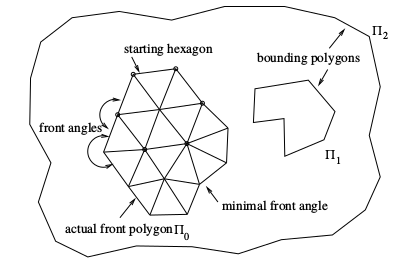
\includegraphics[scale=0.7]{images/hartmann1.png}
	\caption{Nociones básicas del algoritmo de triangulación.}
\end{figure}	
	
	\item[S1] Para cada punto del polígono $\Pi_0$ determinamos el ángulo del área aún por triangular. A estos ángulos los llamamos{ \em ángulos delanteros}.
	
	\begin{figure}[h]
		\centering
		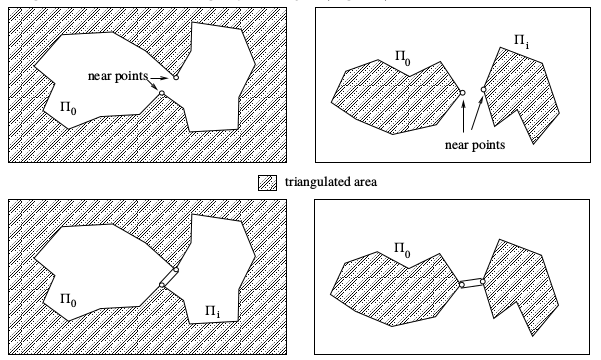
\includegraphics[scale=0.5]{images/hartmann2.png}
		\caption{Dividiendo y uniendo el polígono $\Pi_0$.}
	\end{figure}
	
	\item[S2] Revisamos si algún punto $p_i$ de $\Pi_0$ está cerca. Con cerca entendemos:
	\begin{itemize}
	\item Un punto de $\Pi_0$  distinto de $p_i$ y de su entorno.
	\item Un punto de cualquier otro polígono $\Pi_k$ distinto.
	\end{itemize}
	En el primer caso dividimos el polígono $\Pi_0$ en dos nuevos polígonos $\Pi_0$ y $\Pi_1$. En el segundo caso unimos los dos polígonos en uno nuevo al que llamaremos $\Pi_0$ y será nuestro nuevo polígono delantero actual.
	\item[S3] Determinar un punto $p_m$ del polinomio $\Pi_0$ con un ángulo delantero mínimo. Rodea $p_m$ por triángulos con ángulos cercanos a $\frac{\pi}{6}$. ELimina $p_m$ del polígono $\Pi_0$ e inserta los nuevos puntos en $\Pi_0$.
	\item[S4] Repite los pasos 1, 2 y 3 hasta que $\Pi_0$ consista sólo en tres puntos que generan un nuevo triángulo. Si aún queda algún polígono restante se convierte en el nuevo $\Pi_0$ y se repiten los pasos 1, 2 y 3. Una vez ya no queden más polígonos, habremos terminado y la triangulación estará completada.
\end{enumerate}

\subsubsection{El procedimiento \texttt{surfacepoint}}

Un paso fundamental del algoritmo es determinar el punto $p$ de la superficie que está cerca de un punto $q$ en un entorno de la superficie. El vector $q - p$ no ha de ser necesariamente perpenticular a la superficie. Debido a que casi todas las superficies pueden ser numéricamente implicitadas, daremos a solución para superficies implicitas.
\par Comenzamos con una superficie implícita $\Phi$ definida por una función $f(x) = 0$ para la cual su gradiente $\nabla f$ existe y no se anula para ningún punto de la superficie y un punto $q$ en un entorno de la superficie.
\par El siguiente procedimiento calcula un punto de la superficie $p$, un normal y dos vectores tangentes al punto $p$.

\begin{enumerate}
	\item \begin{itemize}
		\item $u_0 := q$
		\item Repetir $u_{k+1} := u_k - \frac{f(u_k)}{\nabla f(u_k)^2} \nabla f(u_k)$ hasta que $\| u_{k+1} - u_k \|$ es sficientemente pequeño.
		\item $p := u_{k+1}$ 
\end{itemize}		
	\item Definimos el normal a la superficie en $p$ como $n := \frac{\nabla f(p)}{\| \nabla f(p) \|}$.
	\item Para los vectores tangentes: \begin{itemize}
		\item $t_1 := \frac{1}{\| \sqrt{n_x^2 + n_y^2} \|} (n_y, -n_x, 0)$ si $n_x > 0.5$ ó $n_y > 0.5$.
		\item En otro caso elegimos $t_1 := \frac{1}{\| \sqrt{n_x^2 + n_z^2} \|} (-n_z, 0, n_x)$.
		\item $t_2 := n \times t_1$
	\end{itemize}
\end{enumerate}

\subsubsection{La estructura}

Para la construcción de los triángulos necesitamos un paso de longitud $\delta_t > 0$ qie es aproximadamente la longitud de las aristas.
\par Para cada putno $p_i$ guardamos la siguiente información:
\begin{itemize}
	\item Las coordinadas.
	\item El normal y los tangentes a la superficie en $p_i$ tales que son ortonormales entre sí.
	\item El ángulo delantero de $p_i$ si es un punto delantero de $\Pi_0$.
	\item La variable booleana \texttt{angle\_changed} con \texttt{angle\_changed = true} si el ángulo delantero cambió y tiene que ser recalculado.
	\item La variable booleana \texttt{border\_point}, con el valor \texttt{true} si el punto $p_i$ es en el borde de la triangulación y debería ser ignorado para futuros cálculos.
\end{itemize}

Los triángulos serán numerados de forma consecutiva. Para cada triángulo guardaremos el valor numérico de sus vértices.

\subsubsection{S0}

Sea $s$ un punto inicial en un entorno de la superficie. Entonces \texttt{surfacepoint} nos determina el primer punto $p_1$ de la triangulación y el sistema ortonormal $n_1, t_{11} \text{ y } t_{12}$. El resto de puntos $P_2, \dotso, p_7$ son el resultado de aplicar \texttt{surfacepoint} a:

$$q_{i+2} = p_1 + \delta_t cos\left(\frac{i \pi}{3}\right)t_{11} + \delta_t sen\left(\frac{i\pi}{3}\right)t_{12} \hspace{1cm} i = 0, \dotso, 5$$

Ya hemos obtenido los primeros seis triángulos.

\subsubsection{S1}

Si un punto $p_{0i}$ del polígono delantero $\Pi_0 = (p_{01}, \dotso, p_{0N_0})$ acaba de ser incluido o un punto cercano a $p_{0i}$ es un nuevo punto, entonceces es necesario recalcular elángulo delantero $\omega$ del punto $p_{0i}$. Sea:

\begin{itemize}
	\item $v_1 := p_{0,i-1}$ si $i>1$ ó $v_1 := p_{0N_0}$ si $i=1$.
	\item $v_2 := p_{0,i+1}$ si $i<N_0$ ó $v_2 := p_{01}$ si $i=N_0$.
	\item $(\xi_1,\eta_1,\zeta_1)$ y$(\xi_2,\eta_2,\zeta_2)$ las coordenadas de $v_1$ y $v_2$, respectivamente, en el sistema local ortonormal $n, t_1$ y $t_2$ en el punto $p_{0i}$.
	\item $\omega_i$ el ángulo polar de $(\xi_i, \eta_i)$. 
\end{itemize}

Entonces el ángulo delantero en el punto $p_{0i}$ es $\omega = \omega_2 - \omega_1$ si $\omega_2 \geq \omega_1$ ó $\omega = \omega_2 - \omega_1 + 2\pi$ en caso contrario.

\subsubsection{S2}

Para prevenir el solapamiento de nuevos triaángulos sobre los ya existentes comprobaremos:

\begin{itemize}
\item Las distancias dos a dos de los puntos que componen $\Pi_0$. Si hay puntos $p_{0i}$ y $p_{0j}$, con $i<j$, que no son vecinos, ni vecinos de vecino y $\| p_{0i} - p_{0j} \| < \delta_t$ entonces $\Pi_0$ se separa en dos polígonos.
\item Las distancias de puntos de $\Pi_0$ a puntos del resto de polígonos $\Pi_k$. Si hay puntos $p_{0i} \in \Pi_0$ y $p_{mj} \in \Pi_m$ tales que $\| p_{0i} - p_{mj} \| < \delta_t$, entonces los polígonos $\Pi_0$ y $\Pi_m$ se unen.
\end{itemize}

\begin{figure}[h]
\centering
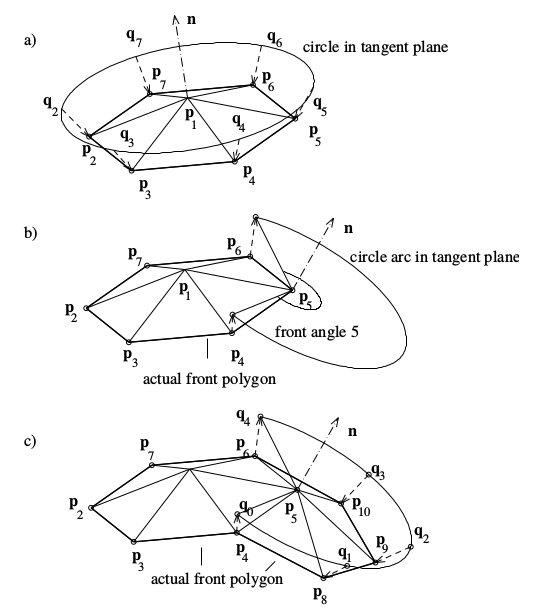
\includegraphics[scale=0.6]{images/hartmann3.png}
\caption{Los primeros pasos del algoritmo.}
\end{figure}

\subsubsection{S3}

Sea $p_{0m}$ un punto de $\Pi_0$  con un ángulo delantero mínimo $\omega$. Completamos la triangulación en $p_{0m}$ de la siguiente manera:

\begin{figure}[h]
\centering
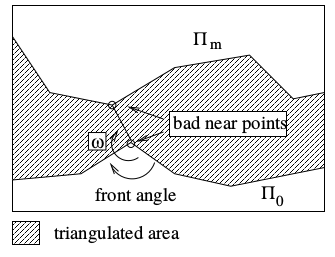
\includegraphics[scale=0.5]{images/hartmann4.png}
\caption{Puntos cercanos \textit{malos} y su detección.}
\end{figure}

\begin{enumerate}
\item Determinamos los vecinos $v_1$ y $v_2$ de $p_{0m}$.
\item Determinamos el número $n_t$ de triángulos que van a ser generados:
$$n_t := \mathtt{trunc}\left( \frac{3\omega}{\pi} \right) + 1 \hspace{1cm} \Delta \omega := \frac{\omega}{n_t}$$
Corrección de $\Delta \omega$ para casos extremos:
\begin{itemize}
\item Si $\Delta \omega < 0.8$ y $n_t > 1$ entonces $n_t \to n_t - 1$ y $\Delta \omega = \frac{\omega}{n_t}$.
\item Si $\Delta \omega < 0.8$, $n_t = 1$ y $\| v_1 - v_2 \| > \frac{5}{4} \delta_t$ entonces $n_t = 2$ y $\Delta \omega \to \frac{\Delta \omega}{2}$.
\item Si $\omega < 3$ y $\| v_1 - p_{0m} \| \leq \frac{1}{2} \delta_t$ (ó $\| v_1 - p_{0m} \| \leq \frac{1}{2} \delta_t$) entonces $n_t = 1$.
\end{itemize}

\begin{figure}[h]
\centering
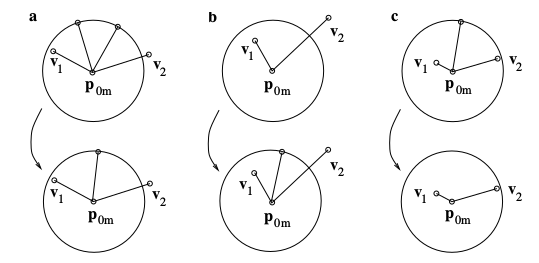
\includegraphics[scale=0.5]{images/hartmann5.png}
\caption{Correcciones de los casos extremos.}
\end{figure}

\item Generamos los triángulos:
\par Si $n_t = 1$ entonces tenemos un nuevo triángulo $(v_1, v_2, p_{0m})$ en otro caso sean $q_0$ y $q_{n_t}$ las proyecciones ortogonales de $v_1$ y $v_2$ en el plano tangente en el punto $p_{0m}$ y sea $q_i$ el resultado de una rotación de ángulo $i \Delta \omega$ alrededor del normal a la superficie en $p_{0m}$ aplicada a $p_{0m} + \delta_t \frac{q_0 - p_{0m}}{\| q_0 - p_{0m} \|}$. Aplicando el procedimiento \texttt{surfacepoint} a $q_i$ obtendremos nuevo puntos $p_{N+i}$ $i = 1, \dotso, n_t -1$, donde $N$ es el total de puntos existentes hasta el momento, y $n_t$ nuevos triángulos.
\item Renovamos el polígono $\Pi_0$:
\par Borramos el punto $p_{0m}$ y, si $n_t > 1$, insertamos en su posición los nuevos puntos $p_{N+1}, \dotso, p_{N+n_t-1}$. Todas las variables booleanas tiene el valor \texttt{true} para asegurarnos de que los nuevos cálculos se realizan.
\end{enumerate}

\subsubsection{Ejemplos de superficies trianguladas}

\textbf{Esfera}
\[\]
Triangulación de la esfera $x^2 + y^2 + z^2 - 4 = 0$ comenzando por el punto $(1,1,1)$ y paso de longitud $\delta_t = 0.3$. La siguiente imagen muestra los primeros cuatro polígonos delanteros y la situación tras 101 y 1531 triángulos. La triangulación total involucra 1534 triángulos.
\[\]
\begin{figure}[h]
\centering
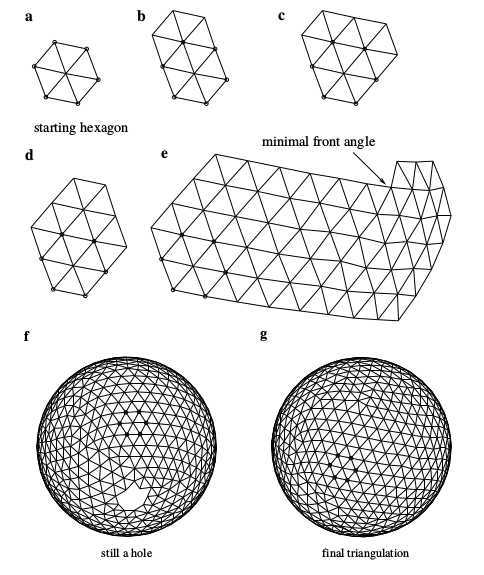
\includegraphics[scale=0.7]{images/hartmann6.png}
\caption{Proceso de triangulación de la esfera.}
\end{figure}

\newpage
\textbf{Cilindro}
\[\]
Triangulación del cilindro $x^2 + y^2 - 1 = 0$ comenzando por el punto $(1,0,0)$ y paso de longitud $\delta_t = 0.2$. 
\[\]
\begin{figure}[h]
\centering
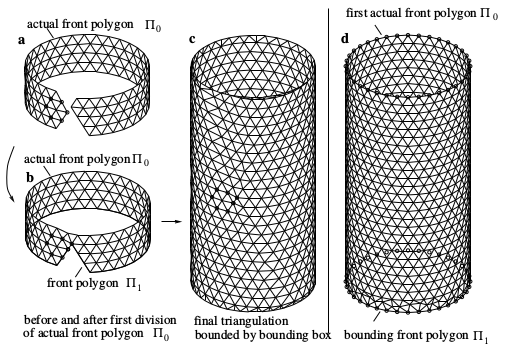
\includegraphics[scale=0.8]{images/hartmann7.png}
\caption{Proceso de triangulación del cilindro.}
\end{figure}

\newpage
\textbf{Toro}
\[\]
Triangulación del cilindro $(x^2+y^2+z^2+0.8775) - 4(x^2+y^2)=0$ comenzando por el punto $(1,0,0.5)$ y paso de longitud $\delta_t = 0.1$.
\[\]

\begin{figure}[h]
\centering
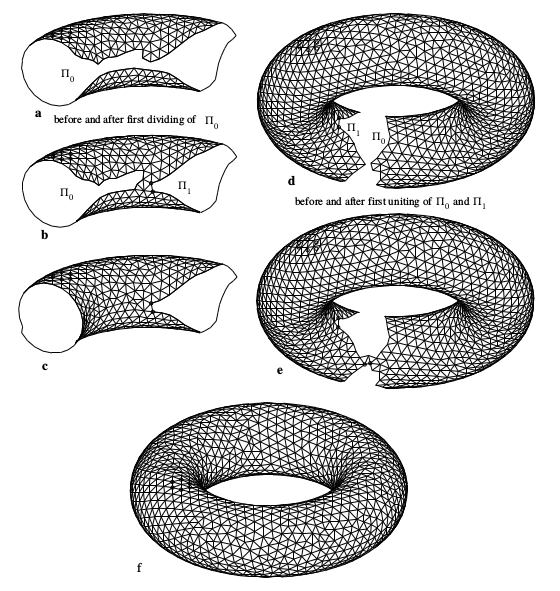
\includegraphics[scale=0.7]{images/hartmann8.png}
\caption{Proceso de triangulación del toro.}
\end{figure}

\newpage
\subsection{Ray Tracing en superficies implícitas}

En 1980, Whitted\cite{Whitted80} propuso un método dpara generar imágenes de alta calidad usando modelos geométricos básicos. Este método evolucionó en lo que hoy se conoce como Ray Tracing, donde la interacción entre rayos de luz y objetos en la nauraleza es simulado: la luz, ya sea artificial o natural, rebota con los objetos y esto es lo que llega a nuestros ojos e interpretamos las propiedades de los objetos, véase color, transparencia, brillo... Además la luz indirecta puede rebotar en varios objetos antes de llegar a nuestros ojos.

\begin{figure}[h]
\centering
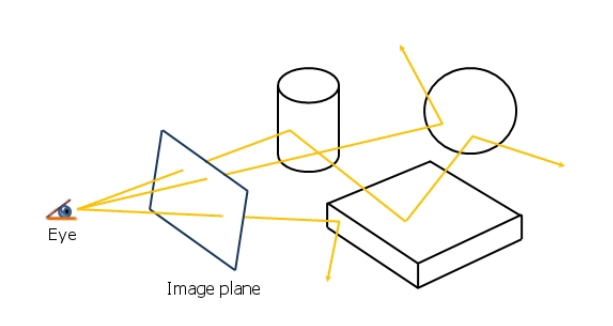
\includegraphics[scale=0.5]{images/florez1.png}
\caption{Rayos de luz rebotando en distintos objetos antes de llegar a nuestros ojos. El plano imagen en la figura se ve cruzado por los rayos; este plano puede contener una representación bidimensional de la escena tridimensional.}
\end{figure}

Usando esta técnica de renderización es posible obtener una representación realista de  de distintos tipos de escenas.
\par En la naturaleza la luz proviene de las llamadas fuentes de luz y, tras rebotar en los objetos del medio, algunos de los rayos llegan a nuestros ojos. Por tanto, analizando el problema, podemos darnos cuenta que, computacionalmente hablando, es muy costoso intentar simular todos los rayos provenientes del foco de luz basándonos en que muchos de los rayos nunca llegarán a nuestro ojo. Por esa razón  es mejor modelar el proceso inverso, esto es, trazar los rayos desde el ojo y buscar las intersecciones con  los objetos del medio.

\subsection{El algoritmo de Ray Tracing}

El método del Ray Tracing es de los llamados{ \em píxel a píxel}. Uno o más rayos de luz son trazados en cada uno de los píxeles en un plano imagen o pantalla. El objetivo es encontrar las intersecciones con los objetos del medio conforme vayamos realizando el trazado de los rayos. Generalmente se suele buscar la primera intersección ya que, en caso de haber más de una, suelen estar obstruidas por el propio objeto.

En la figura \ref{florez27} introducimos el proceso de construcción de un rayo. El punto $c$ representa el origen. Un rayo que comienza en este punto se envía a travez de un píxel en la pantalla con dirección $\vec{cs}$. Estos rayos tienen coordenadas con respecto al sistema $uvw$, mientras que el objeto tiene su propio sistema de referencia $xyz$. Esta independencia de los sistemas de referencia permite ver la escena desde cualquier posición arbitraria.

\begin{figure}[h]
\centering
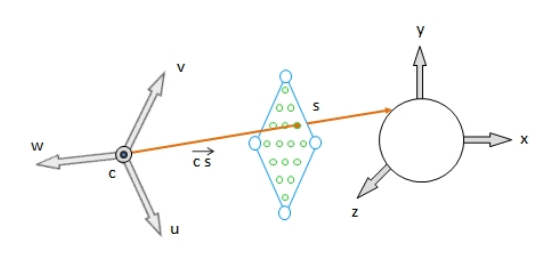
\includegraphics[scale=0.5]{images/florez2.png}
\caption{Definición de un rayo cruzando una pantalla. Si el rayo interseca alguna superficie, el color se calcula y asignado al píxel en la pantalla.}
\label{florez27}
\end{figure}

Si hay alguna intersección entre el rayo y el objeto el color es calculando tomando en cuenta la dirección del vector normal del punto de intersección y la posición de las luces. La aportación de las luces indirectas también se calcula. La suma de todas las posibles aportaciones se usa para asignar el color correspondiente en el píxel.
\[\]
\textbf{Análisis de la intersección}
\[\]
Un rayo se define como:
\begin{equation}
\begin{split}
x = c_x + t(x_s - c_x) \\
y = c_y + t(y_s - c_y) \\
z = c_z + t(y_z - c_z)
\end{split}
\nonumber
\end{equation}

Donde $(c_x,c_y,c_z)$ es origen o punto de vista, $(x_s,y_s,z_s)$ es el punto donde el rayo cruza la pantalla y $t$ es el parámetro del rayo.
\par La intersección entre la superfície implícita $f(x,y,z) = 0$ y el rayo viene definida por la ecuación:

$$g(t) = 0$$

donde $g(t)$ es la función $g : \mathbb{R}_0 \to \mathbb{R}^3$ definida por:

\begin{equation}
g(t) \equiv f(c_x + t(x_s - c_x), c_y + t(y_s - c_y), c_z + t(y_z - c_z))
\nonumber
\end{equation}
De este modo, el problema se reduce a encontrar las raíces de la función $g$.
\par Estas soluciones se sustituyen en la definición parametrica del rayo para encontrar el punto de intersección y el valor del vector normal.
\par Existen muchas maneras  de encontrar las raíces de $g$. Las manera más clásicas son el método de la bisección o de Newton\cite{Hart01}. También existen de otro tipo como: técnicas fuzzy,\cite{Foufou96} aritmética de intervalos\cite{Mitchell90} o constantes de Lipschitz.\cite{Kalra89}

\subsection{Ray Tracing eficiente}

Como ya hemos comentado el principal problema del algoritmo de Ray Tracing es la falta de eficiencia. Muchos autores han propuesto diferentes técnicas de mejora de la eficiencia pero se pueden clasificar en tres grupos:

\begin{itemize}
\item Intersecciones más rápidas.
\item Trazar menor cantidad de rayos.
\item Generalización de los rayos.
\end{itemize}

La técnica más básica para acelerar el Ray Tracing es el llamado{ \em volumen delimitador o límite},que consiste en crear un volumen que contenga a nuestro objeto y que el cálculo de la intersección de los rayos con éste sea menos costoso que con el objeto en sí. La primera propuesta de volumen delimitador fue la esfera\cite{Whitted80} por la simplicidad y por la facilidad para probar la intersección de los rayos con ésta. La idea es recubrir coda objeto con una esfera, si un rayo interseca a una esfera, entonces se analiza el caso dentro de la esfera, en caso contrario no es necesario. Si además añadimos lo que se suele llamar{ \em jerarquía} el orden del algoritmo se puede reducir a $log(n)$.
\par Otra técnica bastante común en la literatura especializada es la subdivisión del espacio en la cual el espacio que rodea a nuestro objeto se divide y se descartan las subdivisiones que no contienen parte del objeto alguno. Podemos dividir el espacio de manera regular o de manera adaptativa como con la poligonalización, pero conlleva los mismos inconvenientes.\\ La ventaja que  tiene este método es que, al ordenar las divisiones, sólo hay que probar el rayo para cada una de éstas en lugar de para el espacio completo para buscar la primera intersección.
\par Ya como final tenemos las llamadas técnicas direccionales en la que se mejora la técnica anterior discretizando también las direcciones.

\section{Conclusiones}

En este capítulo hemos visto distintas maneras de representar y visualizar superficies expresadas de forma implícita, de las cuales ya hemos nombrado sus ventajas e inconvenientes. En términos de coste computacional y velocidad de renderización éstas no presentan ningún reto y presentan una serie de propiedades que las hacen muy atractivas.
\par En el siguiente capítulo haremos una introducción al Análisis de Intervalos para mejorar la capacidad de computación y tratar de solventar los problemas de redondeo de las máquinas debido a los puntos flotantes.
%
%\input{capitulos/03_Planificacion}
%
%\input{capitulos/04_Analisis}
%
%\input{capitulos/05_Diseno}
%
%\input{capitulos/06_Implementacion}
%
%\input{capitulos/07_Pruebas}
%
%\input{capitulos/08_Conclusiones}
%
%\chapter{Conclusiones y Trabajos Futuros}
%
%
\nocite{*}
\bibliography{references}\addcontentsline{toc}{chapter}{Bibliografía}
\bibliographystyle{alpha}
%
%\appendix
%\input{apendices/manual_usuario/manual_usuario}
%%\input{apendices/paper/paper}
%\input{glosario/entradas_glosario}
% \addcontentsline{toc}{chapter}{Glosario}
% \printglossary
%\chapter*{}
%\thispagestyle{empty}

\end{document}
